\begin{figure}
    \centering
    \caption{Seats-Votes Curves for SMC, CRSG, and existing plan.}
    \begin{subfigure}[b]{0.475\textwidth}
        \centering
        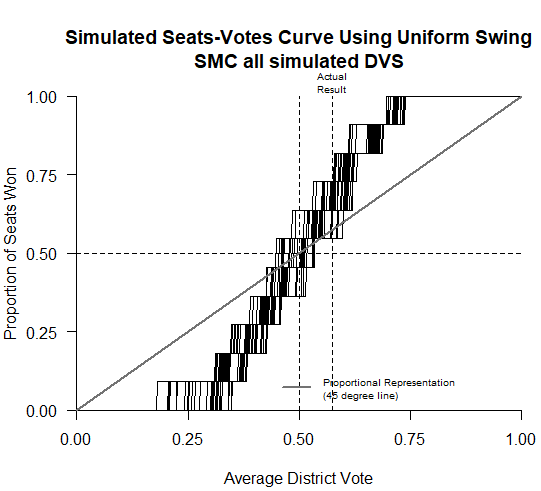
\includegraphics[width=\textwidth]{img/sv.smc.png}
        \caption{SMC Seats-Votes Curve}
        \label{fig:sv.smc}
    \end{subfigure}
    \hfill
    \begin{subfigure}[b]{0.475\textwidth}
        \centering
        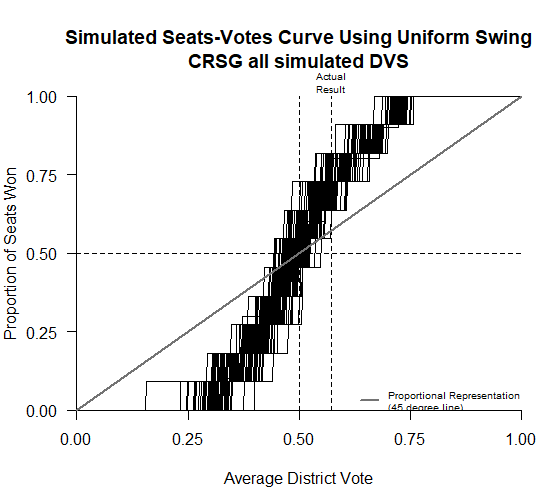
\includegraphics[width=\textwidth]{img/sv.crsg.png}
        \caption{CRSG Seats-Votes Curve}
        \label{fig:sv.crsg}
    \end{subfigure}
    \vskip\baselineskip
    \begin{subfigure}[b]{0.475\textwidth}
        \centering
        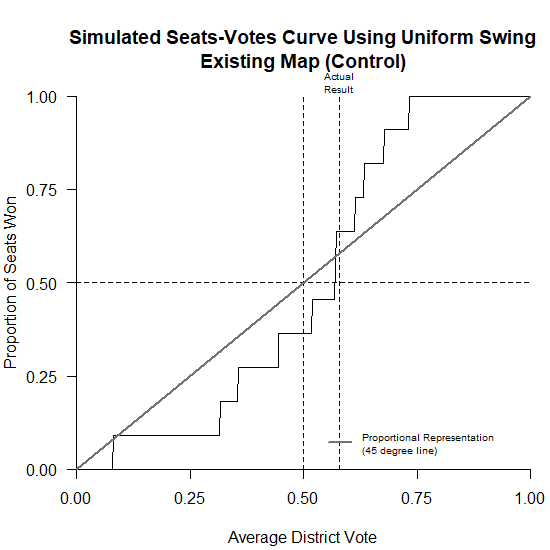
\includegraphics[width=\textwidth]{img/sv.control.png}
        \caption{Real Seats-Votes Curve}
        \label{fig:sv.control}
    \end{subfigure}
    \label{fig:sv}
    \raggedright
    \figurenote{Each plot shows the relationship between average proportion of Democratic vote share by district and the proportion of Democratic seats. Subfigure \ref{fig:sv.smc} illustrates this relationship for the 100 plans generated by SMC, subfigure \ref{fig:sv.crsg} for CRSG, and subfigure \ref{fig:sv.control} is for the existing plan.}
\end{figure}